% MedInfo 2027 full paper: IOS Press book-article class, 5 pages including references.
\documentclass{IOS-Book-Article}
\usepackage[utf8]{inputenc}
\usepackage[T1]{fontenc}
\usepackage{mathptmx}
\usepackage{booktabs}
\usepackage{tikz}
\usetikzlibrary{positioning,arrows.meta,calc,matrix}
% generated by scripts/make_numbers.py; do not edit
\newcommand{\sheetLines}{467,811}
\newcommand{\sheetRows}{633,324}
\newcommand{\sheetNoCode}{165,513}
\newcommand{\sheetRecords}{262,535}
\newcommand{\sheetFixed}{201,394}
\newcommand{\sheetPercent}{61,141}
\newcommand{\sheetAlgorithm}{104,121}
\newcommand{\sheetCollisions}{14,432}
\newcommand{\sheetPayers}{20}
\newcommand{\sheetBatch}{100}
\newcommand{\sheetTx}{1,871}
\newcommand{\sheetSignS}{202}
\newcommand{\sheetSigPerS}{1,852}
\newcommand{\sheetCommitS}{3,090}
\newcommand{\sheetCommitRun}{187,025}
\newcommand{\sheetCommitMin}{72.3}
\newcommand{\sheetRecPerS}{61}
\newcommand{\sheetGas}{310,367}
\newcommand{\sheetBytes}{834}
\newcommand{\sheetCalldataMB}{156}
\newcommand{\sheetDiskMB}{4,711}
\newcommand{\sheetDiskBytes}{17,945}
\newcommand{\sheetLoadS}{572}
\newcommand{\sheetVerifyLines}{363,690}
\newcommand{\sheetVerifyS}{1.3}
\newcommand{\sheetLinesPerS}{289,178}
\newcommand{\sheetCleanMatch}{349,258}
\newcommand{\sheetCleanDiffers}{14,006}
\newcommand{\sheetCleanOther}{426}
\newcommand{\sheetAltered}{3,584}
\newcommand{\sheetCaught}{3,454}
\newcommand{\sheetAlreadyDiffers}{128}
\newcommand{\sheetNotComparable}{2}
\newcommand{\sheetCleanNeedsCM}{426}
\newcommand{\sheetRecPerSEarly}{92}
\newcommand{\sheetRecPerSLate}{48}
\newcommand{\sheetAlready}{75,510}
\newcommand{\sheetDiskBeforeGB}{2.52}
\newcommand{\sheetRepeats}{86,723}
\newcommand{\sheetPctRows}{137,218}
\newcommand{\sheetPctShare}{37.7}
\newcommand{\sheetKeysMulti}{14,292}
\newcommand{\sheetRowsMulti}{30,636}
\newcommand{\projHospitals}{6,000}
\newcommand{\projRecordsB}{1.6}
\newcommand{\projDiskTB}{28}
\newcommand{\projCommitDays}{301}
\newcommand{\pairProviders}{5}
\newcommand{\pairPayerLines}{468}
\newcommand{\pairPayerUnique}{232}
\newcommand{\pairValuesPerKey}{1.53}
\newcommand{\pairAll}{52}
\newcommand{\pairComparable}{33}
\newcommand{\pairNotComparable}{19}
\newcommand{\pairExact}{45.5}
\newcommand{\pairWithinTen}{97.0}
\newcommand{\pairOverFifty}{0.0}
\newcommand{\pairLineComparable}{50}
\newcommand{\pairLineExact}{30.0}
\newcommand{\pairLineAll}{82}
\newcommand{\pairLineWithinTen}{74.0}
\newcommand{\pairLineOverFifty}{4.0}
\newcommand{\pairExactCount}{15}
\newcommand{\coarsePairs}{226}
\newcommand{\coarseComparable}{106}
\newcommand{\coarseNotComparable}{120}
\newcommand{\coarseExact}{14.2}
\newcommand{\coarseWithinTen}{53.8}
\newcommand{\coarseOverFifty}{35.8}
\newcommand{\coarseExactCount}{15}
\newcommand{\sensAsaAllExact}{20.3}
\newcommand{\sensAsaAllWithin}{50.0}
\newcommand{\sensAsaAllOver}{18.9}
\newcommand{\sensAsaAllComparable}{74}
\newcommand{\sensAsaCoarseExact}{7.0}
\newcommand{\sensAsaCoarseOver}{62.6}
\newcommand{\sensAsaCoarseComparable}{214}
\newcommand{\sensDedupAllExact}{28.3}
\newcommand{\sensDedupAllComparable}{46}
\newcommand{\pairWithinFiveCents}{27}
\newcommand{\pairLineExactCI}{19--44}
\newcommand{\coarseExactCI}{9--22}
\newcommand{\sheetBlockS}{4.0}
\newcommand{\sheetSignMinSheet}{4.7}
\newcommand{\sheetTotalMin}{77}
\newcommand{\pairLineExactCount}{15}
\newcommand{\pairRows}{A (Colorado) & 2025-11-01 & 0 & 0 & 44 & 0 & 0 & -- & -- & -- \\
B (Colorado) & 2025-11-01 & 16 & 19 & 73 & 47 & 31 & 35.5 & 58.1 & 6.5 \\
C (Illinois) & 2026-11-03 & 8 & 8 & 16 & 8 & 8 & 37.5 & 100.0 & 0.0 \\
D (Oregon) & 2026-03-23 & 16 & 46 & 24 & 24 & 10 & 0.0 & 100.0 & 0.0 \\
E (California) & 2026-04-01 & 8 & 8 & 18 & 3 & 1 & 100.0 & 100.0 & 0.0 \\}
\newcommand{\pairGroupRows}{Inpatient (8 MS-DRG) & 27 & 17 & 29.4 & 100.0 & 0.0 \\
GI (5 CPT) & 19 & 10 & 70.0 & 90.0 & 0.0 \\
Orthopedic (3 CPT) & 6 & 6 & 50.0 & 100.0 & 0.0 \\}
\newcommand{\synKeys}{28}
\newcommand{\synSigned}{28}
\newcommand{\synProvAltered}{4}
\newcommand{\synPayAltered}{3}
\newcommand{\synBothAltered}{1}
\newcommand{\synExact}{71.4}
\newcommand{\synWithinTen}{78.6}
\newcommand{\synBothMatch}{20}
\newcommand{\synPayerDeparts}{3}
\newcommand{\synProviderDeparts}{4}
\newcommand{\synNeither}{1}
\newcommand{\synProvAlteredAll}{5}
\newcommand{\synPayAlteredAll}{4}
\newcommand{\synUnaltered}{20}

\def\hb{\hbox to 11.5 cm{}}
\tikzset{
  box/.style={draw,rounded corners=2pt,align=center,font=\scriptsize,inner sep=3pt,minimum height=1.6em},
  party/.style={box,fill=black!8},
  file/.style={box,fill=blue!6},
  rec/.style={box,fill=orange!12},
  ledger/.style={box,fill=green!10},
  verdict/.style={box,fill=red!6},
  dec/.style={box,fill=yellow!20},
  lbl/.style={font=\scriptsize,align=center},
  arr/.style={-{Stealth[length=5pt]},thick},
  darr/.style={-{Stealth[length=5pt]},thick,dashed},
}

\begin{document}
\pagestyle{headings}
\def\thepage{}
\begin{frontmatter}
\title{A Permissioned Ledger Framework for Jointly Signed Negotiated Rates Between Providers and Payers}
\markboth{}{\hb}
\author[A]{\fnms{Abhinav} \snm{Srivastava}%
\thanks{Corresponding Author: Abhinav Srivastava, abhinavmirdev@gmail.com.}}
\runningauthor{A. Srivastava}
\address[A]{Independent Researcher}

\begin{abstract}
Under two US rules, hospitals and insurers each publish the prices they negotiated, in separate files, and a 2026 study found both sides published the same price for about 10\% of services. We present CORAL, a permissioned ledger on which the provider and the payer both sign each negotiated rate before either publishes it; a verifier checks each published line against the signed record, and a line that differs marks the file that departs. Signing and committing one provider's full public file, \sheetRecords{} records, took \sheetTotalMin{} minutes on one laptop. Paired on provider and code, five providers' files agreed exactly with one payer's file on \coarseExact\% of comparable prices; paired on the record's fields, on \pairLineExact\%. A synthetic run attributes every altered price in two copies of the signed values to its copy.
\end{abstract}

\begin{keyword}
price transparency\sep negotiated rates\sep blockchain\sep health insurance\sep data integrity
\end{keyword}
\end{frontmatter}
\markboth{\hb}{\hb}

\section{Introduction}

Since 2021, each US hospital must publish a machine-readable file of its standard charges, including the rate negotiated with each payer and plan \cite{hpt}. Since 2022, each group health plan and issuer must publish in-network negotiated rates for every provider \cite{tic}. Each file is produced by one party under its own rule, and neither rule asks the other party to confirm it; the hospital attests to its own file \cite{opps2026}, and from March 2027 the plan attests to its own \cite{tic2026}.

The two sides do not agree. A 2026 industry report compared the files of 450 hospitals with the files of two national payers on 16 common codes: 9.0\% to 11.7\% of pairs matched exactly, 41.7\% to 50.8\% fell within 10\%, and 17.9\% of inpatient pairs differed by more than 50\% \cite{trilliant}. No comparison can say which file is correct, because neither file links a line to a contract version or to the other party.

A negotiated rate is a contract term that two parties agreed. CORAL (Committed Ratesheet on Ledger) is a registry on which a provider and a payer jointly sign each negotiated rate before either publishes it (Figure~1). A verifier with a file and read access to the registry checks each line with one lookup, and a line that departs from the record is attributed to the file that departs. Permissioned ledgers in health care have so far held facts that one party asserts \cite{kuo2017}, and an append to a log proves the sender's action, not the counterparty's agreement \cite{zieglmeier2023}; CORAL puts the counterparty's signature inside the record. We give the record format and the registry contract, sign and commit one provider's full public file, compare five providers' files with one national payer's file on the 16 codes of the 2026 report, and trace synthetic alterations to the copy that carries them. Both signatures in every run come from prototype keys, so the runs show cost and coverage, not that any file is correct.

\begin{figure}[!htb]
\centering
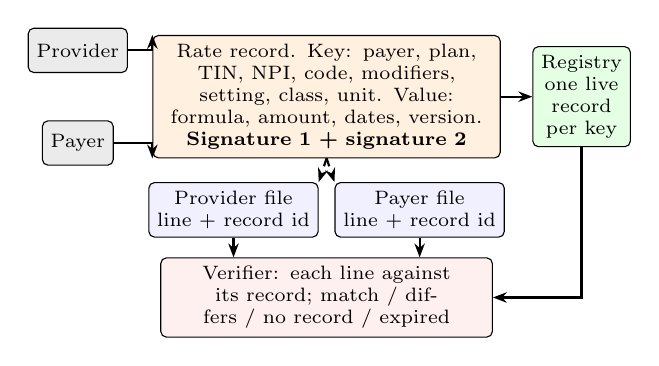
\begin{tikzpicture}[node distance=2.5mm and 4mm]
\node[party] (pb) {Provider};
\node[party, below=6mm of pb] (qb) {Payer};
\node[rec, right=4mm of $(pb.east)!0.5!(qb.east)$, text width=42mm] (rb) {Rate record. Key: payer, plan, TIN, NPI, code, modifiers, setting, class, unit. Value: formula, amount, dates, version. \textbf{Signature 1 + signature 2}};
\node[ledger, right=4mm of rb] (lb) {Registry\\one live\\record\\per key};
\node[file, below=3mm of rb.south, anchor=north east, xshift=-1mm] (fb) {Provider file\\line + record id};
\node[file, below=3mm of rb.south, anchor=north west, xshift=1mm] (gb) {Payer file\\line + record id};
\node[verdict, below=2.5mm of $(fb.south)!0.5!(gb.south)$, text width=40mm] (vb) {Verifier: each line against its record; match / differs / no record / expired};
\draw[arr] (pb.east) -- (rb.west |- pb.east) -- (rb.north west);
\draw[arr] (qb.east) -- (rb.west |- qb.east) -- (rb.south west);
\draw[arr] (rb) -- (lb);
\draw[darr] (rb.south) -- (fb.north east); \draw[darr] (rb.south) -- (gb.north west);
\draw[arr] (fb.south) -- (fb.south |- vb.north);
\draw[arr] (gb.south) -- (gb.south |- vb.north);
\draw[arr] (lb.south) |- (vb.east);
\end{tikzpicture}
\caption{The two parties sign one record per rate, each public file cites it, and a verifier checks each published line against the record; a difference between the files is attributed to the line that departs from the record.}
\end{figure}

\section{Methods}

\textbf{The record.} A rate record has a key and a value. The key identifies one rate: payer id, plan id, provider tax identification number (TIN), billing NPI, billing code and type, modifiers, setting (inpatient, outpatient, or both), billing class (facility or professional), and drug unit. Each key field maps to a field of the CMS hospital CSV format and of the Transparency in Coverage JSON schema \cite{schemas}; the payer file's place-of-service codes give the setting, because its own setting field reads ``both'' on nearly every price. The value gives the formula (fixed amount, percent of charges, or percent of a reference schedule), the amount, the start and end dates, a contract version, the chargemaster version a percent rate applies to, and the record this one supersedes.

\textbf{Identity and keys.} The provider's root is its TIN, the level at which contracts are signed and which the payer file carries; the payer's root is the party that holds the contract, by HIOS issuer id or EIN. A registrar, CMS in the prototype, binds an entity id to a root key once and never signs a rate. Each entity holds its root key offline and delegates signing keys to the system that produces its rate sheet. Validity is judged at the block timestamp of the commit, which the signer cannot choose, and a revocation takes effect at or after the block that carries it, so it cannot be backdated to before a record its key committed. Root replacement after loss is proposed by the registrar, takes effect after seven days, and the current root can veto it.

\textbf{The registry.} The registry is one contract on a permissioned Ethereum-compatible network. Each action carries EIP-712 typed-data signatures bound to the chain id and contract address; both parties sign the same structure hash, and that hash is the record id. One record is live per key: a new record whose window overlaps a live record is rejected unless it names that record in its supersedes field, and the old record then ends where the new one starts. The prototype network is Hyperledger Besu 26.10.2 with IBFT 2.0 consensus, a two-second block period, and four validators standing for CMS, a provider association, a payer association, and an auditor; validators order transactions and cannot sign a rate. All four ran in containers on one laptop (10-core ARM, 64 GB) with full state history kept, so the figures carry no network latency and include archive storage.

\textbf{Verification.} A verifier reads the registry once into an index by key and checks each published line with one lookup: the signed amount for a fixed rate, the signed percent or its product with the line's list price for a percent-of-charges rate. A pair of lines from the two files resolves to both match, payer file departs, provider file departs, both depart, or unsigned.

\textbf{Full-sheet run.} We take the public file of provider A, a hospital in Colorado (dated 2025-11-01, CMS format 3.0.0); providers are lettered A to E and payers are not named. Every row with a percentage becomes a percent-of-charges record, every other row with a dollar amount a fixed record; rows with only an algorithm are counted. One record is signed per key, from the first row in file order; a later row with the same key and a different value is a key collision. We verify every row with a standard code and a value against the registry, and again after altering 1\% of those rows in the field the record signs.

\textbf{Pair run on real data.} We take five providers' files and one in-network file of a national commercial payer, payer P (one plan cluster, dated 2026-10-05, 547 plans, 1.69 GB compressed). For each provider we keep the rows for payer P's commercial plans on the 16 codes of the 2026 report, with a manual plan crosswalk listed in the code, and from the payer file the prices for the providers' NPIs on the same codes, pooled at the TIN level. We pair the files twice: on provider and code alone, as a comparison without the record key must; and on the record key, every provider line against every distinct payer value of its key. Each measure reports exact match, within 10\%, and more than 50\% apart over pairs where both sides give the same kind of value.

\textbf{Synthetic attribution.} For each paired key with a provider dollar amount we sign one record with that amount, build a provider copy and a payer copy of the signed value, alter each line of each copy independently with probability 0.1, verify both copies, and report the attribution. The run tests the attribution step only. All code, the contract, the parsers, and the run output are public \cite{repo}.

\section{Results}

\textbf{Full-sheet run.} The file has \sheetRows{} rows. \sheetNoCode{} carry only a chargemaster, revenue, or NDC code and are outside the record format; the remaining \sheetLines{} rows name \sheetPayers{} payers, and \sheetAlgorithm{} give an algorithm and no value. The \sheetVerifyLines{} rows with a value reduce to \sheetRecords{} records, \sheetFixed{} fixed and \sheetPercent{} percent of charges; \sheetCollisions{} rows (4.0\% of rows with a value) carry a different value for a key already signed, on \sheetKeysMulti{} keys. Signing both sides took \sheetSignS{} s (\sheetSigPerS{} signatures per second). Commits ran \sheetBatch{} records per transaction at \sheetRecPerS{} records per second over the run (\sheetCommitMin{} minutes), falling from \sheetRecPerSEarly{} over the first 20,000 records to \sheetRecPerSLate{} over the last 50,000. Each record took \sheetDiskBytes{} bytes of validator storage, \sheetDiskMB{} MB for the sheet. Verification of the clean file returned \sheetCleanMatch{} matches and \sheetCleanDiffers{} amount-differs and \sheetCleanNeedsCM{} needs-chargemaster verdicts, all on collision keys, in \sheetVerifyS{} s. In the altered copy, \sheetAltered{} rows changed; \sheetCaught{} moved from match to amount differs, \sheetAlreadyDiffers{} were collision rows that differed before, and \sheetNotComparable{} were needs-chargemaster rows.

\textbf{Pair run on real data.} Payer P's file lists \pairPayerLines{} prices for the five providers' NPIs on the 16 codes, \pairPayerUnique{} after duplicates merge. Paired on provider and code alone, the files give \coarsePairs{} pairs, \coarseComparable{} comparable; \coarseExactCount{} (\coarseExact\%, 95\% interval \coarseExactCI\%) matched exactly, \coarseWithinTen\% fell within 10\%, and \coarseOverFifty\% differed by more than 50\%. Paired on the record key, there are \pairLineAll{} pairs, \pairLineComparable{} comparable, of which \pairLineExactCount{} (\pairLineExact\%, interval \pairLineExactCI\%) matched exactly, \pairLineWithinTen\% fell within 10\%, and \pairLineOverFifty\% differed by more than 50\% (Table~1). The payer file rounds to ten cents; \pairWithinFiveCents{} of the \pairLineComparable{} agree within five cents. Provider A has no pair: its rows for payer P on these codes are all Medicare Advantage, outside the Transparency in Coverage rule. Provider B gives 31 of the \pairLineComparable{} comparable pairs; with its leased-network product line included, the key pairing gives \sensAsaAllExact\% exact on \sensAsaAllComparable{} pairs.

\begin{table}[!htb]
\caption{Five providers against payer P's file on the 16 codes of the 2026 report, paired on the record key. Provider files dated 2025-11-01 to 2026-11-03. Percentages are of comparable pairs.}
\centering
\scriptsize
\setlength{\tabcolsep}{2.5pt}
\begin{tabular}{lrrrrrrr}
\toprule
Provider & Provider keys & Payer keys & Pairs & Comparable & Exact \% & Within 10\% & Over 50\% \\
\midrule
\pairRowsShort
\bottomrule
\end{tabular}
\end{table}

\textbf{Synthetic attribution and key rotation.} \synKeys{} paired keys had a provider dollar amount. The alteration touched \synProvAlteredAll{} provider copies and \synPayAlteredAll{} payer copies: \synProvAltered{} keys had only the provider copy changed, \synPayAltered{} only the payer copy, and \synBothAltered{} both. Verification attributed \synProviderDeparts{} differences to the provider copy, \synPayerDeparts{} to the payer copy, and \synNeither{} to both; the \synUnaltered{} unaltered keys matched on both sides. On the running network, a commit with a revoked signing key reverted and the same commit with the newly delegated key succeeded; the earlier record stayed valid, and a backdated revocation reverted.

\section{Discussion}

The record format holds every row of a real provider file with a standard code and a value, and the key fields of the public formats identify a rate for all but \sheetCollisions{} rows; those are items that share a billing code but differ in list price and fixed amount, which a key extended with the provider's item code would separate. Paired on provider and code, the five files and payer P's file reproduce the 2026 report within a few points; paired on the fields the record carries, the over-50\% share falls from \coarseOverFifty\% to \pairLineOverFifty\% and the exact share doubles. The large disagreements the report measures therefore lie mostly in fields the record carries, and what remains after pairing on the record key is what a signed record would attribute to one file. The sample is \pairLineComparable{} key pairs from four providers against one payer, and the files differ in date, so part of the disagreement can be a rate update.

\textbf{Scale and design.} About \projHospitals{} hospitals with a sheet of this size give \projRecordsB{} billion records; at the measured storage and rate that is about \projDiskTB{} TB per validator and \projCommitDays{} days of commits, before any payer-side record. A pruned state profile was not measured; a deployment can store the record id and the two signatures only. Kuo and colleagues' conditions for a ledger apply \cite{kuo2017}: several parties record the same term, the history must be append-only, and no party is accepted by the others as operator. A CMS-run signed log would give the same inclusion guarantee with no consensus layer; whether replication is worth having is a governance question this paper does not settle. Three of four validators can rewrite history and every validator reads every record before publication; a deployment needs more validators with opposed interests and read access set as policy.

\textbf{Adoption and limitations.} The second signature does not exist today. The hospital rule could require that a reported rate cite a jointly signed record, as the CY2026 rule extended the attestation \cite{opps2026}; a payer has its own reason to ask for the record, as a defense against a provider file that overstates a rate. Where the parties do not agree a value, no record exists and the files carry the disagreement in the open. Both signatures in every run come from prototype keys, so no run shows that a file is correct, only that a file matches the record it was minted from. The record covers fixed, percent-of-charges, and percent-of-reference rates and not lesser-of clauses, outliers, carve-outs, bundles, escalators, algorithm-only rows, or leased networks. The registry cannot detect a rate that both parties signed wrongly.

\section{Conclusions}

The record format covers every row of a real provider file with a standard code and a value, and signing and committing the sheet took \sheetTotalMin{} minutes on one laptop. Five providers' files agree exactly with one payer's on \coarseExact\% of comparable pairs when paired on provider and code and on \pairLineExact\% when paired on the record key. With a jointly signed record behind each rate, a verifier attributes a difference to the file that departs; no comparison of the two files can do that today.

\begin{thebibliography}{99}
\footnotesize\setlength{\itemsep}{0pt}
\bibitem{hpt} Centers for Medicare \& Medicaid Services. Price Transparency Requirements for Hospitals To Make Standard Charges Public. Final rule. Fed Regist. 2019 Nov 27;84(229):65524--606. Codified at 45 CFR Part 180.
\bibitem{tic} Internal Revenue Service, Employee Benefits Security Administration, Centers for Medicare \& Medicaid Services. Transparency in Coverage. Final rule. Fed Regist. 2020 Nov 12;85(219):72158--310.
\bibitem{opps2026} Centers for Medicare \& Medicaid Services. Medicare Program: Hospital Outpatient Prospective Payment and Ambulatory Surgical Center Payment Systems (CY 2026). Final rule. Fed Regist. 2025 Nov 25;90:53448. CMS-1834-FC.
\bibitem{tic2026} Internal Revenue Service, Employee Benefits Security Administration, Centers for Medicare \& Medicaid Services. Transparency in Coverage. Final rules. Fed Regist. 2026 Oct 6;91(192):63748--867. TD 10058; CMS-9882-F.
\bibitem{trilliant} Patton K, Ikard M, Browne J, Oakes A. The majority of hospital and health plan reported rates diverge by more than 10\% [Internet]. Trilliant Health; 2026 Apr 30 [cited 2026 Nov 3]. Available from: https://www.trillianthealth.com/market-research/studies/the-majority-of-hospital-and-health-plan-reported-rates-diverge-by-more-than-10
\bibitem{kuo2017} Kuo TT, Kim HE, Ohno-Machado L. Blockchain distributed ledger technologies for biomedical and health care applications. J Am Med Inform Assoc. 2017;24(6):1211--20, doi:10.1093/jamia/ocx068
\bibitem{zieglmeier2023} Zieglmeier V. Appending data to blockchain is not sufficient for non-repudiation of receipt. arXiv:2308.04781 [cs.CR]. 2023 Aug 9.
\bibitem{schemas} Centers for Medicare \& Medicaid Services. Hospital price transparency CSV data dictionary v3.0; Transparency in coverage in-network rate schema [Internet]. [cited 2026 Nov 3]. Available from: https://github.com/CMSgov
\bibitem{repo} Srivastava A. CORAL: Committed Ratesheet on Ledger [source code]. 2026. Available from: https://github.com/AbhinavMir/coral
\end{thebibliography}
\end{document}
